\documentclass[aspectratio=169,10pt]{beamer}

% A concise 15-minute technical presentation based on UIO_IFAC.tex.
\usefonttheme{professionalfonts}
\usepackage[T1]{fontenc}
\usepackage[utf8]{inputenc}
% Use scalable outline fonts.  The bitmap EC fonts produced by the default
% T1 setup can be clipped by Edge's PDF renderer at some full-screen zooms.
\usepackage{lmodern}
\usepackage{amsmath,amssymb,bm,mathtools}
\usepackage{booktabs}
\usepackage{graphicx}
\usepackage{tikz}
\usetikzlibrary{arrows.meta,positioning,fit,calc}

% Ask browser PDF viewers to show one complete slide at a time.  In
% particular, this avoids the last page being bottom-aligned and cropped in
% Edge's continuous full-screen view.
\hypersetup{pdfstartview=Fit,pdfpagelayout=SinglePage}

\graphicspath{{../img/}{../}}

\definecolor{ifacblue}{RGB}{17,91,140}
\definecolor{ifaccyan}{RGB}{0,145,170}
\definecolor{ifacgreen}{RGB}{35,126,98}
\definecolor{ifacink}{RGB}{31,42,55}
\definecolor{ifacmuted}{RGB}{102,113,128}
\definecolor{ifaclight}{RGB}{242,247,250}
\definecolor{ifacline}{RGB}{211,222,230}

\setbeamercolor{normal text}{fg=ifacink,bg=white}
\setbeamercolor{structure}{fg=ifacblue}
\setbeamercolor{frametitle}{fg=ifacink,bg=white}
\setbeamercolor{title}{fg=ifacblue}
\setbeamercolor{subtitle}{fg=ifacmuted}
\setbeamercolor{block title}{fg=white,bg=ifacblue}
\setbeamercolor{block body}{fg=ifacink,bg=ifaclight}
\setbeamercolor{alerted text}{fg=ifaccyan}
\setbeamercolor{author in head/foot}{fg=ifacmuted}
\setbeamercolor{date in head/foot}{fg=ifacmuted}
\setbeamerfont{title}{series=\bfseries,size=\LARGE}
\setbeamerfont{subtitle}{size=\large}
\setbeamerfont{frametitle}{series=\bfseries,size=\Large}
\setbeamerfont{footline}{size=\scriptsize}
\setbeamertemplate{navigation symbols}{}
\setbeamertemplate{itemize item}{\color{ifacblue}$\blacktriangleright$}
\setbeamertemplate{itemize subitem}{\color{ifaccyan}$\bullet$}
\setlength{\leftmargini}{1.3em}
\setlength{\leftmarginii}{1.1em}

% Speaker notes ---------------------------------------------------------------
% A normal compilation creates the slide-only audience PDF.
% UIO_IFAC_15min_presenter_notes.tex defines \presenternotes before loading this
% file and creates the side-by-side PDF expected by Pympress (--notes=right).
\newif\ifshownotes
\ifdefined\presenternotes
  \shownotestrue
\else
  \shownotesfalse
\fi
\ifshownotes
  \setbeameroption{show notes on second screen=right}
\else
  \setbeameroption{hide notes}
\fi
\newcommand{\speakernote}[1]{\note{\scriptsize #1}}
\setbeamertemplate{note page}{%
  \vbox to \paperheight{%
    \vskip0.45cm
    \hbox to \paperwidth{\hskip0.60cm\begin{minipage}[t]{0.87\paperwidth}\color{ifacblue}\large\bfseries\insertframetitle\end{minipage}\hfill}%
    \vskip0.14cm
    \hbox to \paperwidth{\hskip0.60cm\color{ifacline}\rule{0.87\paperwidth}{0.45pt}\hfill}%
    \vskip0.28cm
    \hbox to \paperwidth{\hskip0.60cm\begin{minipage}{0.87\paperwidth}\color{ifacink}\insertnote\end{minipage}\hfill}%
    \vfill
  }%
}

\setbeamertemplate{frametitle}{%
  \vspace{0.34cm}%
  \hspace{0.55cm}\insertframetitle\par
  \vspace{0.10cm}\hspace{0.55cm}\color{ifacline}\rule{0.94\textwidth}{0.45pt}%
}
\setbeamertemplate{footline}{%
  \vspace{0.05cm}\hspace{0.55cm}\color{ifacmuted}\insertshorttitle
  \hfill\insertframenumber\,/\,\inserttotalframenumber\hspace{0.55cm}\vspace{0.18cm}%
}

\newcommand{\R}{\mathbb{R}}
\newcommand{\Hone}{\mathcal H^1}
\newcommand{\Ltwo}{\mathcal L_2}
\newcommand{\norm}[1]{\left\lVert #1\right\rVert}
\newcommand{\T}{\mathsf T}
\newcommand{\vect}[1]{\bm{#1}}

\tikzset{
  block/.style={draw=ifacblue, very thick, rounded corners=2pt, fill=ifaclight,
    minimum height=0.95cm, align=center, text width=2.9cm, inner sep=4pt},
  smallblock/.style={draw=ifacblue, thick, rounded corners=2pt, fill=ifaclight,
    minimum height=0.74cm, align=center, text width=2.15cm, inner sep=3pt},
  learnblock/.style={draw=ifacgreen, very thick, rounded corners=2pt, fill=ifacgreen!8,
    minimum height=0.95cm, align=center, text width=2.9cm, inner sep=4pt},
  flow/.style={-Latex, very thick, draw=ifacblue},
  learnflow/.style={-Latex, very thick, draw=ifacgreen},
  signal/.style={font=\scriptsize\color{ifacmuted}, midway, fill=white, inner sep=1.5pt}
}

% Reused first as the global roadmap, then repeated at the Layer-2 transition.
\newcommand{\teacherarchitecture}{%
  \vspace{0.12cm}
  \centering
  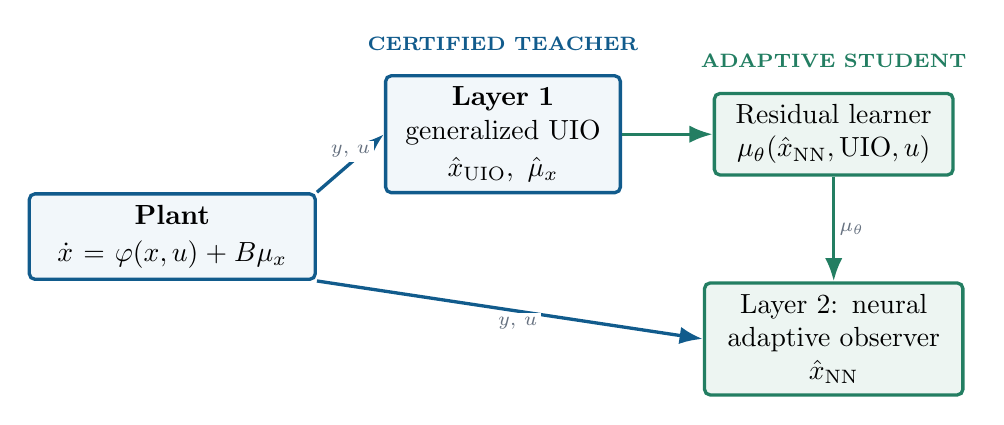
\begin{tikzpicture}
    \node[block, text width=3.35cm] (plant) at (-0.30,0)
      {\textbf{Plant}\\[0.5mm]$\dot x=\varphi(x,u)+B\mu_x$};
    \node[block, text width=2.70cm] (uio) at (3.90,1.30)
      {\textbf{Layer 1}\\generalized UIO\\[0.5mm]
       $\hat x_{\rm UIO},\ \hat\mu_x$};
    \node[learnblock, text width=2.75cm] (model) at (8.10,1.30)
      {Residual learner\\$\mu_\theta(\hat x_{\rm NN},\mathrm{UIO},u)$};
    \node[learnblock, text width=3.00cm] (nao) at (8.10,-1.30)
      {Layer 2: neural adaptive observer\\$\hat x_{\rm NN}$};

    \node[font=\scriptsize\bfseries\color{ifacblue}, above=0.18cm of uio]
      {CERTIFIED TEACHER};
    \node[font=\scriptsize\bfseries\color{ifacgreen}, above=0.18cm of model]
      {ADAPTIVE STUDENT};

    \draw[flow] (plant.north east) --
      node[signal, pos=.50, above] {$y,\,u$} (uio.west);
    \draw[learnflow] (uio.east) -- (model.west);
    \draw[learnflow] (model.south) --
      node[signal, pos=.50, right] {$\mu_\theta$} (nao.north);
    \draw[flow] (plant.south east) --
      node[signal, pos=.52, below] {$y,\,u$} (nao.west);
  \end{tikzpicture}

  \vspace{0.28cm}
  \scriptsize\textcolor{ifacblue}{\textbf{Teacher:}} bounded, physics-based supervisory signals
  \hspace{1.6em}
  \textcolor{ifacgreen}{\textbf{Student:}} adaptive residual learning
}

\title[Learning with Unknown Input Observers]{Learning with Unknown Input Observers\\for Robust Nonlinear Estimation}
\subtitle{A hybrid, certified estimator for systems with unknown dynamics}
\author{Q. H. Nguyen \and L. Qi \and A. Zemouche \and H. Rafaralahy \and M. Haddad}
\institute{IFAC 2026}
\date{}

\begin{document}

% -----------------------------------------------------------------------------
\begin{frame}[plain]
  \vspace{0.52cm}
  \begin{columns}[T,onlytextwidth]
    \begin{column}{0.73\textwidth}
      \hspace{0.35cm}\begin{minipage}{0.95\linewidth}
        \raggedright
        {\color{ifacblue}\Large\bfseries
          Learning with Unknown Input\\Observers for Robust\\Nonlinear Estimation\par}
        \vspace{0.25cm}
        {\usebeamercolor[fg]{subtitle}\usebeamerfont{subtitle}\insertsubtitle\par}
        \vspace{0.72cm}
        {\small Q. H. Nguyen \quad L. Qi \quad A. Zemouche \quad H. Rafaralahy \quad M. Haddad\par}
        \vspace{0.22cm}
        {\color{ifacmuted}\insertinstitute\par}
        \vspace{0.88cm}
        \color{ifacblue}\rule{\linewidth}{1.3pt}\par
        \vspace{0.22cm}
        \hbox to \linewidth{%
          \hfill
          \raisebox{0.07cm}{
\includegraphics[height=0.42cm,keepaspectratio]{../fig/image001.png}}%
          \hspace{0.55cm}%
          
\includegraphics[height=0.62cm,keepaspectratio]{../fig/R.png}%
          \hfill
        }
      \end{minipage}
    \end{column}
    \begin{column}{0.23\textwidth}
      \vspace{-0.18cm}
      \centering
      
\includegraphics[height=0.75\textheight,keepaspectratio]{../fig/IFAC_2026_banner.png}
    \end{column}
  \end{columns}
  \speakernote{
    \textbf{Memory cue:} Brief welcome, name, and title.\par\smallskip
    Good morning everyone, and thank you for joining us. I am Quang Huy Nguyen, and today I will present our work on learning with unknown input observers for robust nonlinear estimation.
  }
\end{frame}

% -----------------------------------------------------------------------------
\begin{frame}{Global architecture: certified estimation guides learning}
\teacherarchitecture
\speakernote{
  \textbf{Memory cue:} State the core idea through the complete architecture.\par\smallskip
  Let me begin with the core idea and the global view. Our physical model is nonlinear, and part of its dynamics is unknown. Instead of asking one estimator to do everything, we combine a certified model-based observer with an adaptive learning layer.\par\smallskip
  From left to right, the measured output and known input first feed the generalized UIO. This certified teacher estimates both the state $\hat x_{\rm UIO}$ and the unknown input $\hat\mu_x$. These bounded, physics-based signals supervise the residual learner. The learned residual $\mu_\theta$ is then injected into Layer 2, a neural adaptive observer that propagates its own state estimate $\hat x_{\rm NN}$ and remains anchored to the measurements.\par\smallskip
  This is the roadmap for the talk: first I will construct and certify Layer 1; then I will return to this architecture to explain the Layer-2 observer and its online learning loop; finally, I will show the vehicle results.
}
\end{frame}

% -----------------------------------------------------------------------------
\begin{frame}{Why estimation becomes difficult with unknown dynamics}
\begin{columns}[T,onlytextwidth]
  \begin{column}{0.53\textwidth}
    \vspace{0.15cm}
    \begin{block}{Nonlinear plant with an unknown input}
      \vspace{-0.15cm}
      \begin{align*}
        \dot{x} &= \varphi(x,u)+B\mu_x, & x&\in\R^{n_x},\\[-1mm]
        y &= Cx, & \mu_x&\in\R^{n_\mu}.
      \end{align*}
      \vspace{-0.32cm}
    \end{block}
    \vspace{0.18cm}
    \small
    \begin{itemize}
      \item $\varphi(x,u)$: known nonlinear physics;
      \item $\mu_x$: unmodelled dynamics, disturbances, or force residuals;
      \item only $y$ is measured and $\mu_x$ must be inferred online.
    \end{itemize}
  \end{column}
  \begin{column}{0.42\textwidth}
    \vspace{0.08cm}
    \centering
    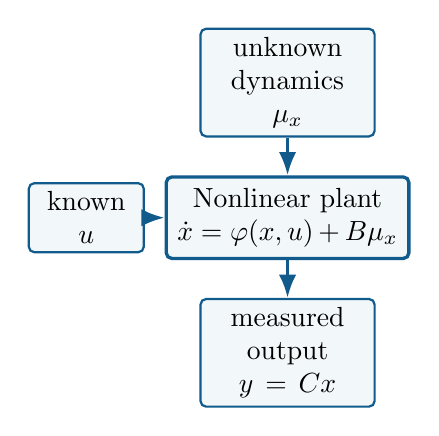
\begin{tikzpicture}[node distance=0.48cm]
      \node[block, text width=2.8cm] (plant) {Nonlinear plant\\$\dot x=\varphi(x,u)+B\mu_x$};
      \node[smallblock, text width=1.25cm, left=0.25cm of plant] (input) {known\\$u$};
      \node[smallblock, text width=2.0cm, above=of plant] (unknown) {unknown dynamics\\$\mu_x$};
      \node[smallblock, text width=2.0cm, below=of plant] (output) {measured output\\$y=Cx$};
      \draw[flow] (input) -- (plant);
      \draw[flow] (unknown) -- (plant);
      \draw[flow] (plant) -- (output);
    \end{tikzpicture}
    \par\vspace{0.20cm}
    {\small\textcolor{ifaccyan}{\textbf{Goal:}} estimate $x$ and infer $\mu_x$.\par}
  \end{column}
\end{columns}
\speakernote{
  \textbf{Memory cue:} Known physics plus an unknown input. Estimate both the state and the residual.\par\smallskip
  Let us start from the model on this slide. The state evolves according to the known nonlinear physics, written as $\varphi(x,u)$, plus an unknown input $B\mu_x$. We measure only $y=Cx$.\par\smallskip
  The term $\mu_x$ collects what the nominal model does not explain: unmodelled dynamics, disturbances, or force residuals. The difficulty is that this term affects the state, but it is not directly measured. Therefore, a good estimator should reconstruct the physical state robustly and provide a useful estimate of the unknown input. Classical unknown-input observer theory is useful, but it also reveals its main limitation.
}
\end{frame}

% -----------------------------------------------------------------------------
\begin{frame}{The classical UIO condition is often too restrictive}
\begin{columns}[T,onlytextwidth]
  \begin{column}{0.52\textwidth}
    \vspace{0.28cm}
    \begin{block}{Direct unknown-input decoupling requires}
      \[
        \operatorname{rank}(CB)=\operatorname{rank}(B).
      \]
    \end{block}
    \vspace{0.22cm}
    \begin{itemize}
      \item This guarantees that the output is informative enough to isolate $\mu_x$.
      \item In real vehicle and robotic systems, $CB$ can be rank deficient.
      \item Enforcing exact decoupling can then rule out an otherwise useful observer.
    \end{itemize}
  \end{column}
  \begin{column}{0.43\textwidth}
    \vspace{0.35cm}
    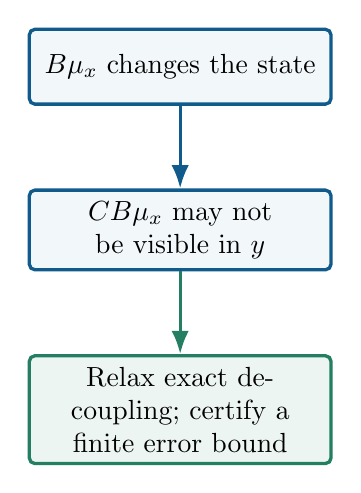
\begin{tikzpicture}[node distance=1.05cm]
      \node[block, text width=3.55cm] (rank) {$B\mu_x$ changes the state};
      \node[block, text width=3.55cm, below=of rank] (cb) {$CB\mu_x$ may not be visible in $y$};
      \node[learnblock, text width=3.55cm, below=of cb] (goal) {Relax exact decoupling; certify a finite error bound};
      \draw[flow] (rank) -- (cb);
      \draw[learnflow] (cb) -- (goal);
    \end{tikzpicture}
  \end{column}
\end{columns}
\speakernote{
  \textbf{Memory cue:} Classical UIO needs rank. Real systems often do not give it.\par\smallskip
  A conventional unknown-input observer relies on the rank condition shown here: the rank of $CB$ must equal the rank of $B$. Intuitively, the measured output must contain enough information to separate the effect of the unknown input from the state dynamics.\par\smallskip
  When this condition holds, an observer can exactly decouple the unknown input and obtain exponential convergence. However, this assumption is often too strong in practice. A sensor set may not see every direction in which an unknown tire force, disturbance, or model mismatch acts. In that case, $CB$ can be rank deficient. Instead of discarding the observer design, our approach relaxes exact decoupling and replaces it with a quantified estimation bound.
}
\end{frame}

% -----------------------------------------------------------------------------
\begin{frame}{Regularization converts a rank obstacle into a bounded disturbance}
\begin{columns}[T,onlytextwidth]
  \begin{column}{0.63\textwidth}
    \vspace{0.08cm}
    \small
    \begin{align*}
      \dot{x}+E_{\delta_1}\dot\mu_x
        &=\varphi(x,u)+B\mu_x+E\omega_{\delta_1},\\[-1mm]
      y&=Cx+D_{\delta_2}\mu_x+D\omega_{\delta_2},\\[-1mm]
      E_{\delta_1}&=\delta_1E,\qquad D_{\delta_2}=\delta_2D,\\[-1mm]
      \omega_{\delta_1}&=\delta_1\dot\mu_x,\qquad
      \omega_{\delta_2}=-\delta_2\mu_x.
    \end{align*}
    \vspace{-0.17cm}
    \begin{itemize}
      \item The transformed model is equivalent to the original plant.
      \item The tunable $\delta_1,\delta_2$ restore observer design freedom.
      \item The price is explicit: $\omega_\delta$ enters the performance analysis.
    \end{itemize}
  \end{column}
  \begin{column}{0.32\textwidth}
    \vspace{0.50cm}
    \begin{block}{Certified consequence}
      \vspace{-0.25cm}
      \[
      \norm{\tilde\zeta}_{\Hone}
      \leq \lambda_\delta\norm{\mu_x}_{\Hone}
      +\beta\norm{\xi_0}.
      \]
      \vspace{-0.10cm}
    \end{block}
    \vspace{0.22cm}
    \centering
    \textcolor{ifacgreen}{\textbf{Exact convergence}} is recovered when the classical rank condition holds.
  \end{column}
\end{columns}
\speakernote{
  \textbf{Memory cue:} Do not force exact decoupling; make the remaining effect measurable and bounded.\par\smallskip
  The key step is a regularized reformulation of the original system. We introduce the tunable quantities $\delta_1$ and $\delta_2$, and write an equivalent model in which the derivative of the unknown input and the unknown input itself appear through the disturbance vector $\omega_\delta$.\par\smallskip
  This does not change the underlying plant. The regularization creates enough freedom to construct an observer even when the direct rank condition is not available. The cost is explicit: the unknown-input effect enters the performance analysis. The inequality on the right says that the augmented-state estimation error is bounded in the $\mathcal H^1$ norm by the unknown dynamics and by the initial estimation error. If the classical rank condition is available, the regularization can be removed and exact convergence is recovered.
}
\end{frame}

% -----------------------------------------------------------------------------
\begin{frame}{Output derivatives create a generalized unknown-input observer}
\begin{columns}[T,onlytextwidth]
  \begin{column}{0.60\textwidth}
    \vspace{0.05cm}
    \small
    Introduce $\chi_1=y$ and $\chi_2=\dot y$ in the augmented state
    $\zeta=\begin{bmatrix}\chi_1^\T&\chi_2^\T&x^\T&\mu_x^\T\end{bmatrix}^\T$:
    \begin{align*}
      \dot\chi_1&=\chi_2,\\[-1mm]
      \dot\chi_2&=C\bar\varphi_x(x,u)
        +C\frac{\partial\varphi}{\partial x}(x,u)B\mu_x+CB\dot\mu_x,\\[-1mm]
      \dot{x}&=\varphi(x,u)+B\mu_x,\\[-1mm]
      y_\chi&=\chi_1+C_\chi\chi_2+Cx.
    \end{align*}
  \end{column}
  \begin{column}{0.35\textwidth}
    \vspace{0.22cm}
    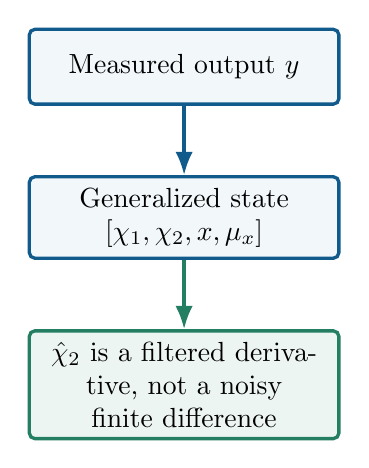
\begin{tikzpicture}[node distance=0.88cm]
      \node[block, text width=3.65cm] (y) {Measured output $y$};
      \node[block, text width=3.65cm, below=of y] (g) {Generalized state\\$[\chi_1,\chi_2,x,\mu_x]$};
      \node[learnblock, text width=3.65cm, below=of g] (deriv) {$\hat\chi_2$ is a filtered derivative, not a noisy finite difference};
      \draw[flow] (y) -- (g);
      \draw[learnflow] (g) -- (deriv);
    \end{tikzpicture}
  \end{column}
\end{columns}
\speakernote{
  \textbf{Memory cue:} Augment with output derivatives, but estimate them through the observer.\par\smallskip
  To strengthen the information available to the observer, we introduce the output and its derivative as auxiliary variables: $\chi_1=y$ and $\chi_2=\dot y$. These variables are included with the state and unknown input in one generalized augmented state.\par\smallskip
  The derivative channel brings additional information about the nonlinear dynamics and the unknown input. We do not take a noisy numerical derivative of the measurement. The generalized observer estimates $\chi_2$ internally, so $\hat\chi_2$ behaves as a filtered output derivative. This gives more information without the usual finite-difference noise amplification. With this model, we can synthesize the first certified estimation layer.
}
\end{frame}

% -----------------------------------------------------------------------------
\begin{frame}{Layer 1: LMI-certified generalized UIO}
\begin{columns}[T,onlytextwidth]
  \begin{column}{0.51\textwidth}
    \vspace{0.04cm}
    \begin{block}{Observer realization}
      \vspace{-0.22cm}
      \begin{align*}
        \dot\eta&=P_\zeta\varphi_\zeta(\hat\zeta,u)
          +K(y-\mathcal H\hat\zeta),\\[-1mm]
        \hat\zeta&=\eta+Q_\zeta y,\qquad
        P_\zeta\mathcal E+Q_\zeta\mathcal H=I.
      \end{align*}
      \vspace{-0.32cm}
    \end{block}
    \vspace{0.17cm}
    \[
      K=\mathcal P^{-1}\mathcal Q^\T.
    \]
    \vspace{-0.07cm}
    \begin{alertblock}{Guarantee}
      Feasibility yields an $\Hone$ estimation bound for the state and unknown input.
    \end{alertblock}
  \end{column}
  \begin{column}{0.46\textwidth}
    \vspace{0.12cm}
    \small
    For every vertex $j$ of the nonlinear embedding, solve
    \[
      \left[
      \begin{array}{ccc}
        \Xi_j & \Gamma_j & \Theta_j\\
        \Gamma_j^\T & -\lambda I_{2n_\mu} & \Gamma_j^\T\\
        \Theta_j^\T & \Gamma_j & -\epsilon^{-1}\mathcal P
      \end{array}
      \right]\prec0.
    \]
    \vspace{0.16cm}
    \begin{itemize}
      \item offline convex synthesis;
      \item online observer with a quantified robustness level $\lambda_\delta$.
    \end{itemize}
  \end{column}
\end{columns}
\speakernote{
  \textbf{Memory cue:} Offline LMI, online robust observer.\par\smallskip
  This slide gives the first-layer observer. Its estimated augmented state $\hat\zeta$ contains the output-related variables, the physical state, and the unknown input estimate. The matrices $P_\zeta$ and $Q_\zeta$ enforce the structural decoupling relation, while the gain $K$ is computed from the LMI solution.\par\smallskip
  The LMI is solved offline at the vertices of the nonlinear embedding, which turns the gain design into a convex feasibility problem. Once it is feasible, Layer 1 has an $\mathcal H^1$ estimation guarantee. It is therefore not only an estimator, but also a source of supervisory signals whose robustness can be quantified before deployment. This reliability is exactly what we need before introducing learning.
}
\end{frame}

% -----------------------------------------------------------------------------
\begin{frame}{A certified teacher supervises learning}
\teacherarchitecture
\speakernote{
  \textbf{Memory cue:} Layer 1 teaches; Layer 2 learns the part that the fixed model misses.\par\smallskip
  This diagram summarizes the hybrid architecture. The plant provides the measured output and receives the known input. Layer 1, the generalized UIO, estimates both the state $\hat x_{\rm UIO}$ and the unknown residual $\hat\mu_x$.\par\smallskip
  These quantities are passed to the neural approximation. They act as a teacher signal: they are not assumed to be perfect, but they are bounded and physically meaningful because they come from the certified observer. Layer 2 is the neural adaptive observer. It uses the neural approximation together with measurement feedback to refine the state estimate. The first layer protects learning with a robust baseline; the second captures state-dependent effects that a fixed observer model cannot represent as well.
}
\end{frame}

% -----------------------------------------------------------------------------
\begin{frame}{Layer 2: a neural observer estimates its own state}
\begin{columns}[T,onlytextwidth]
  \begin{column}{0.55\textwidth}
    \vspace{0.05cm}
    \small
    \begin{block}{State-dependent residual model}
      \vspace{-0.20cm}
      \begin{align*}
        \mu_\theta(\hat x_{\rm NN})
        =\mathcal N_\theta\!\left(
        \hat x_{\rm NN},\hat x_{\rm UIO},\hat\mu_x,u\right).
      \end{align*}
      \vspace{-0.32cm}
    \end{block}
    \vspace{0.16cm}
    \begin{block}{Layer-2 observer dynamics}
      \vspace{-0.24cm}
      \begin{align*}
        \dot{\hat x}_{\rm NN}
          &=\varphi(\hat x_{\rm NN},u)
            +B\mu_\theta(\hat x_{\rm NN})
            +L_{\rm NN}(y-y_{\rm NN}),\\[-1mm]
        y_{\rm NN}&=C\hat x_{\rm NN}.
      \end{align*}
      \vspace{-0.32cm}
    \end{block}
    \vspace{0.01cm}
    \scriptsize
    The UIO supplies supervisory inputs; it does not replace the independent
    dynamic state $\hat x_{\rm NN}\in\R^{n_x}$.
  \end{column}
  \begin{column}{0.40\textwidth}
    \vspace{0.05cm}
    \begin{block}{Three contributions to $\dot{\hat x}_{\rm NN}$}
      \small
      \begin{itemize}
        \item known nonlinear physics $\varphi$;
        \item learned unknown dynamics $B\mu_\theta$;
        \item measurement innovation $L_{\rm NN}(y-y_{\rm NN})$.
      \end{itemize}
    \end{block}
    \vspace{0.01cm}
    \begin{alertblock}{Certified error channel}
      \scriptsize
      With $\epsilon_{\rm NN}=x-\hat x_{\rm NN}$ and
      $\Delta_x=\mu_x-\mu_\theta$,
      \vspace{-0.05cm}
      \begin{align*}
        \dot\epsilon_{\rm NN}
        &=\bigl(\nabla_x^\varphi-L_{\rm NN}C\bigr)
          \epsilon_{\rm NN}+B\Delta_x,\\[-1mm]
        \norm{\epsilon_{\rm NN}}_{\Ltwo}
        &\leq\lambda_{\rm NN}\norm{\Delta_x}_{\Ltwo}
          +\beta_{\rm NN}\norm{\epsilon_{\rm NN}(0)}.
      \end{align*}
      \vspace{-0.25cm}
    \end{alertblock}
  \end{column}
\end{columns}
\speakernote{
  \textbf{Memory cue:} Layer 2 is an observer with its own state, not only a neural correction block.\par\smallskip
  The neural model takes the current Layer-2 estimate together with the UIO state estimate, the UIO unknown-input estimate, and the known input. It predicts the state-dependent residual $\mu_\theta$.\par\smallskip
  Crucially, Layer 2 propagates its own state $\hat x_{\rm NN}$. Its dynamics combine the known nonlinear physics, the learned residual through $B\mu_\theta$, and the measurement innovation through $L_{\rm NN}(y-y_{\rm NN})$. Subtracting this observer from the plant gives the error dynamics on the right. The remaining approximation error $\Delta_x$ is the input to the certified $\mathcal L_2$ bound. The next slide explains how online learning reduces this mismatch.
}
\end{frame}

% -----------------------------------------------------------------------------
\begin{frame}{Layer 2: online parameter adaptation}
\vspace{0.02cm}
\centering
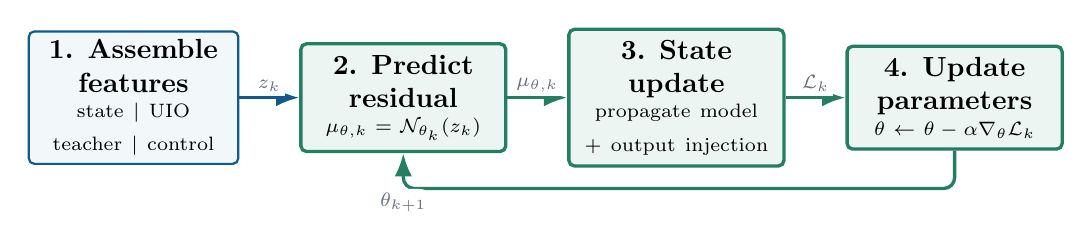
\begin{tikzpicture}[node distance=0.76cm]
  \node[smallblock, text width=2.45cm, minimum height=1.14cm] (features)
    {\textbf{1. Assemble features}\\[-1mm]
     \scriptsize state $\mid$ UIO teacher $\mid$ control};
  \node[learnblock, text width=2.32cm, minimum height=1.14cm, right=of features] (network)
    {\textbf{2. Predict residual}\\[-1mm]
     \scriptsize $\mu_{\theta,k}=\mathcal N_{\theta_k}(z_k)$};
  \node[learnblock, text width=2.45cm, minimum height=1.14cm, right=of network] (observer)
    {\textbf{3. State update}\\[-1mm]
     \scriptsize propagate model $+$ output injection};
  \node[learnblock, text width=2.45cm, minimum height=1.14cm, right=of observer] (update)
    {\textbf{4. Update parameters}\\[-1mm]
     \scriptsize $\theta\leftarrow\theta-\alpha\nabla_\theta\mathcal L_k$};
  \draw[flow] (features) -- node[signal, above] {$z_k$} (network);
  \draw[learnflow] (network) -- node[signal, above] {$\mu_{\theta,k}$} (observer);
  \draw[learnflow] (observer) -- node[signal, above] {$\mathcal L_k$} (update);
  \draw[learnflow, rounded corners=4pt] (update.south) -- ++(0,-0.48cm) -|
    node[signal, pos=.52, below] {$\theta_{k+1}$} (network.south);
\end{tikzpicture}

\vspace{0.08cm}
\begin{columns}[T,onlytextwidth]
  \begin{column}{0.57\textwidth}
    \small
    \begin{block}{Composite objective at sample $k$}
      \vspace{-0.27cm}
      \begin{align*}
        \mathcal L_k={}&\norm{\hat x_{{\rm NN},k}-x_{{\rm ref},k}}_{T_{\rm ref}}^2
        +\norm{y_k-C\hat x_{{\rm NN},k}}_{T_y}^2\\[-1mm]
        &+\norm{\hat x_{{\rm NN},k}-\hat x_{{\rm UIO},k}}_{T_{\rm UIO}}^2
        +\lambda\norm{\mu_{\theta,k}-\hat\mu_{x,k}}^2.
      \end{align*}
      \vspace{-0.34cm}
    \end{block}
    \scriptsize
    The four terms respectively promote reference tracking, measurement consistency,
    agreement with the UIO, and residual matching to the teacher proxy.
  \end{column}
  \begin{column}{0.38\textwidth}
    \small
    \begin{block}{Features and parameter update}
      \scriptsize
      \begin{align*}
        z_k={}&\operatorname{col}(\hat x_{{\rm NN},k},
          \hat x_{{\rm UIO},k},\hat\mu_{x,k},u_k),\\[-1mm]
        \mu_{\theta,k}={}&\mathcal N_{\theta_k}(z_k),\\[-1mm]
        \theta_{k+1}={}&\theta_k-\alpha_k
          \nabla_\theta\mathcal L_k,\qquad \alpha_k>0.
      \end{align*}
      \vspace{-0.08cm}
      The LMI-designed observer gain $L_{\rm NN}$ remains fixed while the network
      parameters adapt online to reduce $\Delta_x$.
    \end{block}
  \end{column}
\end{columns}
\speakernote{
  \textbf{Memory cue:} Learn the residual, keep output feedback, and bound the remaining mismatch.\par\smallskip
  The feature vector collects the current neural-state estimate, the UIO state estimate, the UIO unknown-input estimate, and the known input. The network produces $\mu_{\theta,k}$, which enters the state observer shown on the previous slide.\par\smallskip
  The four loss terms promote reference tracking, measurement consistency, agreement with the certified UIO teacher, and residual matching to the teacher proxy. Gradient descent updates only the neural parameters. The LMI-designed innovation gain remains fixed, so online adaptation reduces the residual mismatch without changing the certified observer structure.
}
\end{frame}

% -----------------------------------------------------------------------------
\begin{frame}{Case study: nonlinear vehicle with unknown tire forces}
\begin{columns}[T,onlytextwidth]
  \begin{column}{0.53\textwidth}
    \vspace{0.16cm}
    \begin{block}{Vehicle state, input, and measurement}
      \vspace{-0.20cm}
      \begin{align*}
        x&=\begin{bmatrix}v_x&v_y&\psi&r\end{bmatrix}^{\T},
        &u&=\begin{bmatrix}a&\delta\end{bmatrix}^{\T},\\[-1mm]
        y&=\begin{bmatrix}v_x&\psi&r\end{bmatrix}^{\T},
        &\mu_x&=\begin{bmatrix}f_{y f}&f_{y r}\end{bmatrix}^{\T}.
      \end{align*}
      \vspace{-0.30cm}
    \end{block}
    \begin{itemize}
      \item Lateral velocity $v_y$ is not directly measured.
      \item Front/rear lateral tire-force residuals represent the unknown input.
      \item A layered controller provides the manoeuvring input used by both estimators.
    \end{itemize}
  \end{column}
  \begin{column}{0.42\textwidth}
    \vspace{0.10cm}
    \centering
    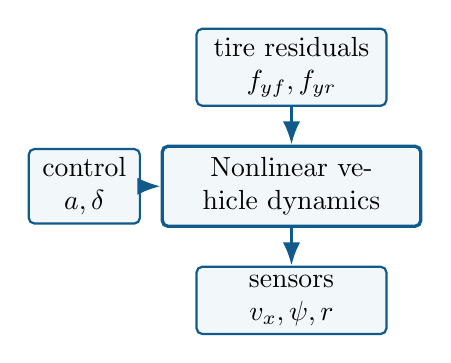
\begin{tikzpicture}[node distance=0.48cm]
      \node[block, text width=3.0cm] (vehicle) {Nonlinear vehicle dynamics};
      \node[smallblock, text width=1.20cm, left=0.25cm of vehicle] (ctrl) {control\\$a,\delta$};
      \node[smallblock, text width=2.2cm, above=of vehicle] (tire) {tire residuals\\$f_{yf},f_{yr}$};
      \node[smallblock, text width=2.2cm, below=of vehicle] (sensors) {sensors\\$v_x,\psi,r$};
      \draw[flow] (ctrl) -- (vehicle);
      \draw[flow] (tire) -- (vehicle);
      \draw[flow] (vehicle) -- (sensors);
    \end{tikzpicture}
  \end{column}
\end{columns}
\speakernote{
  \textbf{Memory cue:} Unmeasured lateral velocity and unknown front--rear tire-force residuals.\par\smallskip
  We evaluate the method on a nonlinear vehicle model. The state contains longitudinal velocity, lateral velocity, yaw angle, and yaw rate. The known inputs are acceleration and steering angle. The measured output contains longitudinal velocity, yaw angle, and yaw rate, so the lateral velocity $v_y$ is not measured directly.\par\smallskip
  The unknown input is composed of the front and rear lateral tire-force residuals. These residuals represent the difference between the nominal tire model and the effective forces needed to explain the motion. The vehicle setting illustrates the broader problem: use known physics where it is reliable, then estimate and learn the structured dynamics that are missing.
}
\end{frame}

% -----------------------------------------------------------------------------
\begin{frame}{Trajectory tracking: centimetre-scale position error}
\begin{columns}[T,onlytextwidth]
  \begin{column}{0.68\textwidth}
    \centering
    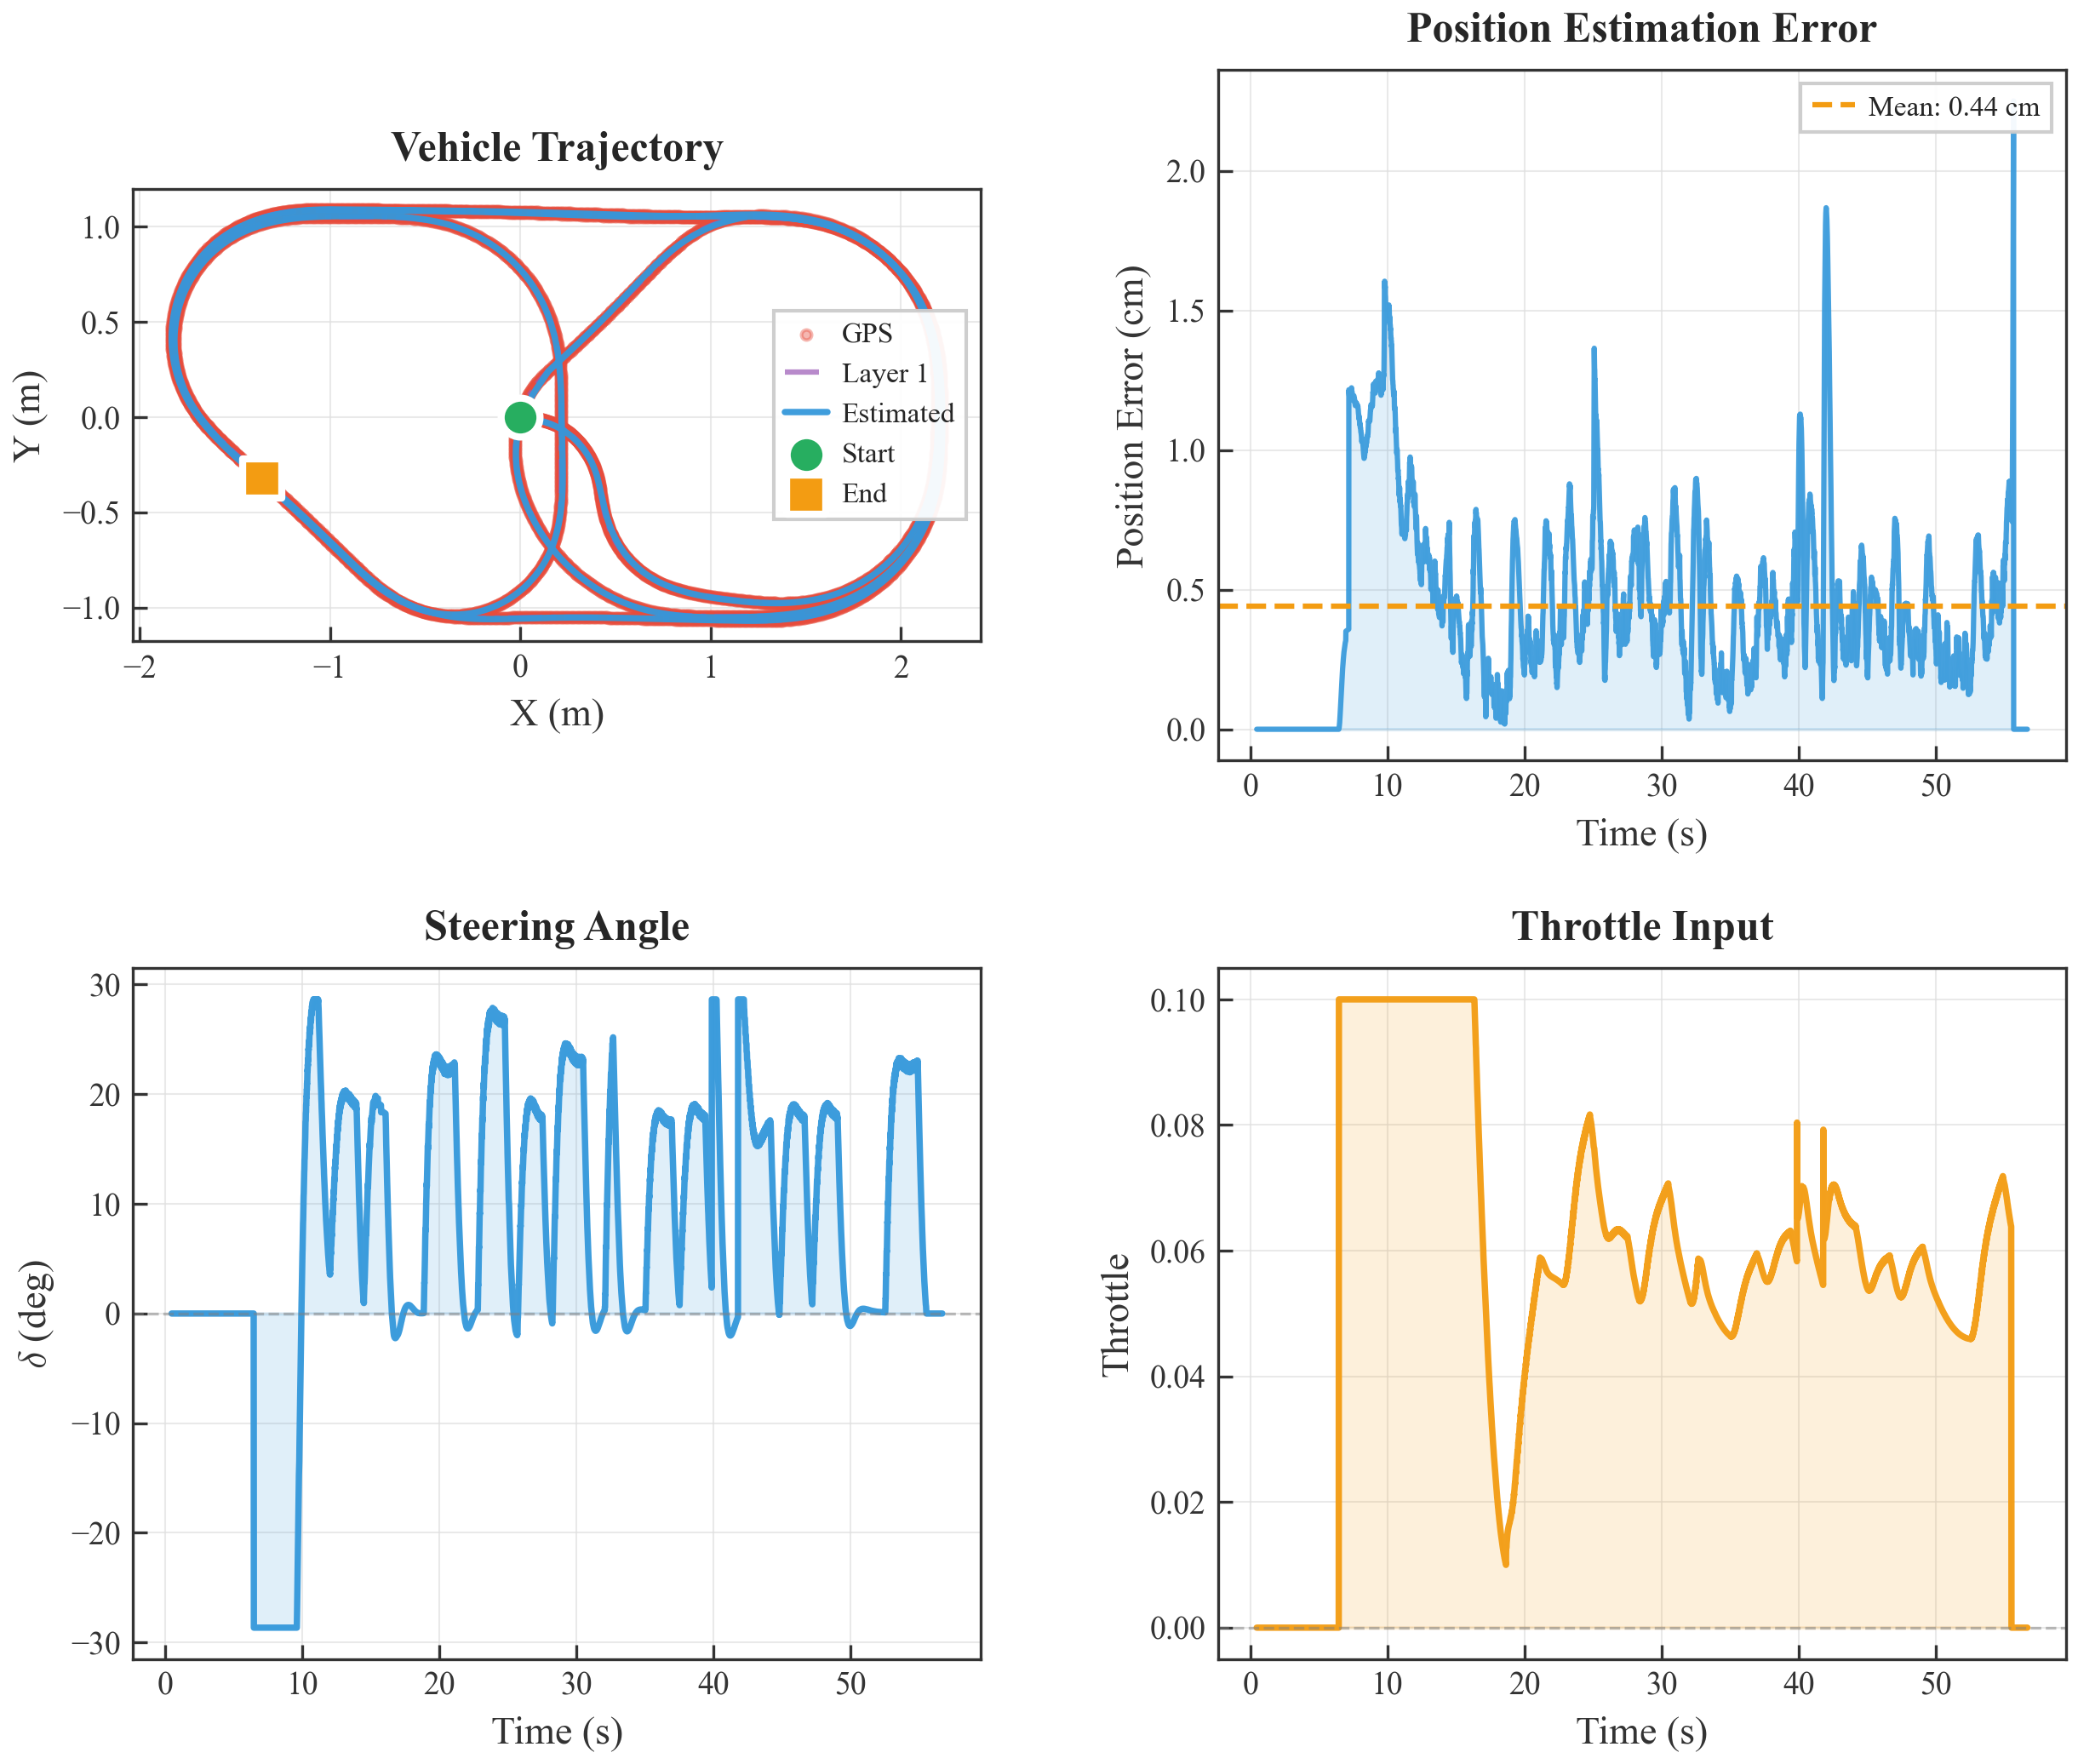
\includegraphics[width=0.96\linewidth,height=0.67\textheight,keepaspectratio]{traj_control_py.png}
  \end{column}
  \begin{column}{0.28\textwidth}
    \vspace{0.28cm}
    \begin{block}{Observed outcome}
      The estimated trajectory closely follows the GPS reference during the manoeuvre.
    \end{block}
    \vspace{0.23cm}
    \begin{alertblock}{Reported metric}
      Mean position error: \textbf{0.44 cm}.
    \end{alertblock}
    \vspace{0.18cm}
    The lower panel confirms feasible steering and acceleration commands.
  \end{column}
\end{columns}
\speakernote{
  \textbf{Memory cue:} First practical result: the estimated path follows GPS closely.\par\smallskip
  First, consider the trajectory result. In the upper-left plot, the estimated trajectory closely follows the GPS reference throughout the manoeuvre. This means that the combined estimator remains consistent at the position level, even while it handles nonlinear dynamics and unknown tire-force effects.\par\smallskip
  The upper-right plot reports the position error. The mean position error is 0.44 centimetres in this simulation. The key point is not only the small average value; it is also the absence of a sustained drift. The lower plots show steering and throttle inputs, confirming that this performance is achieved during a manoeuvre with changing control inputs rather than in a static operating condition.
}
\end{frame}

% -----------------------------------------------------------------------------
\begin{frame}{State estimation: the unmeasured lateral velocity is reconstructed}
\begin{columns}[T,onlytextwidth]
  \begin{column}{0.69\textwidth}
    \centering
    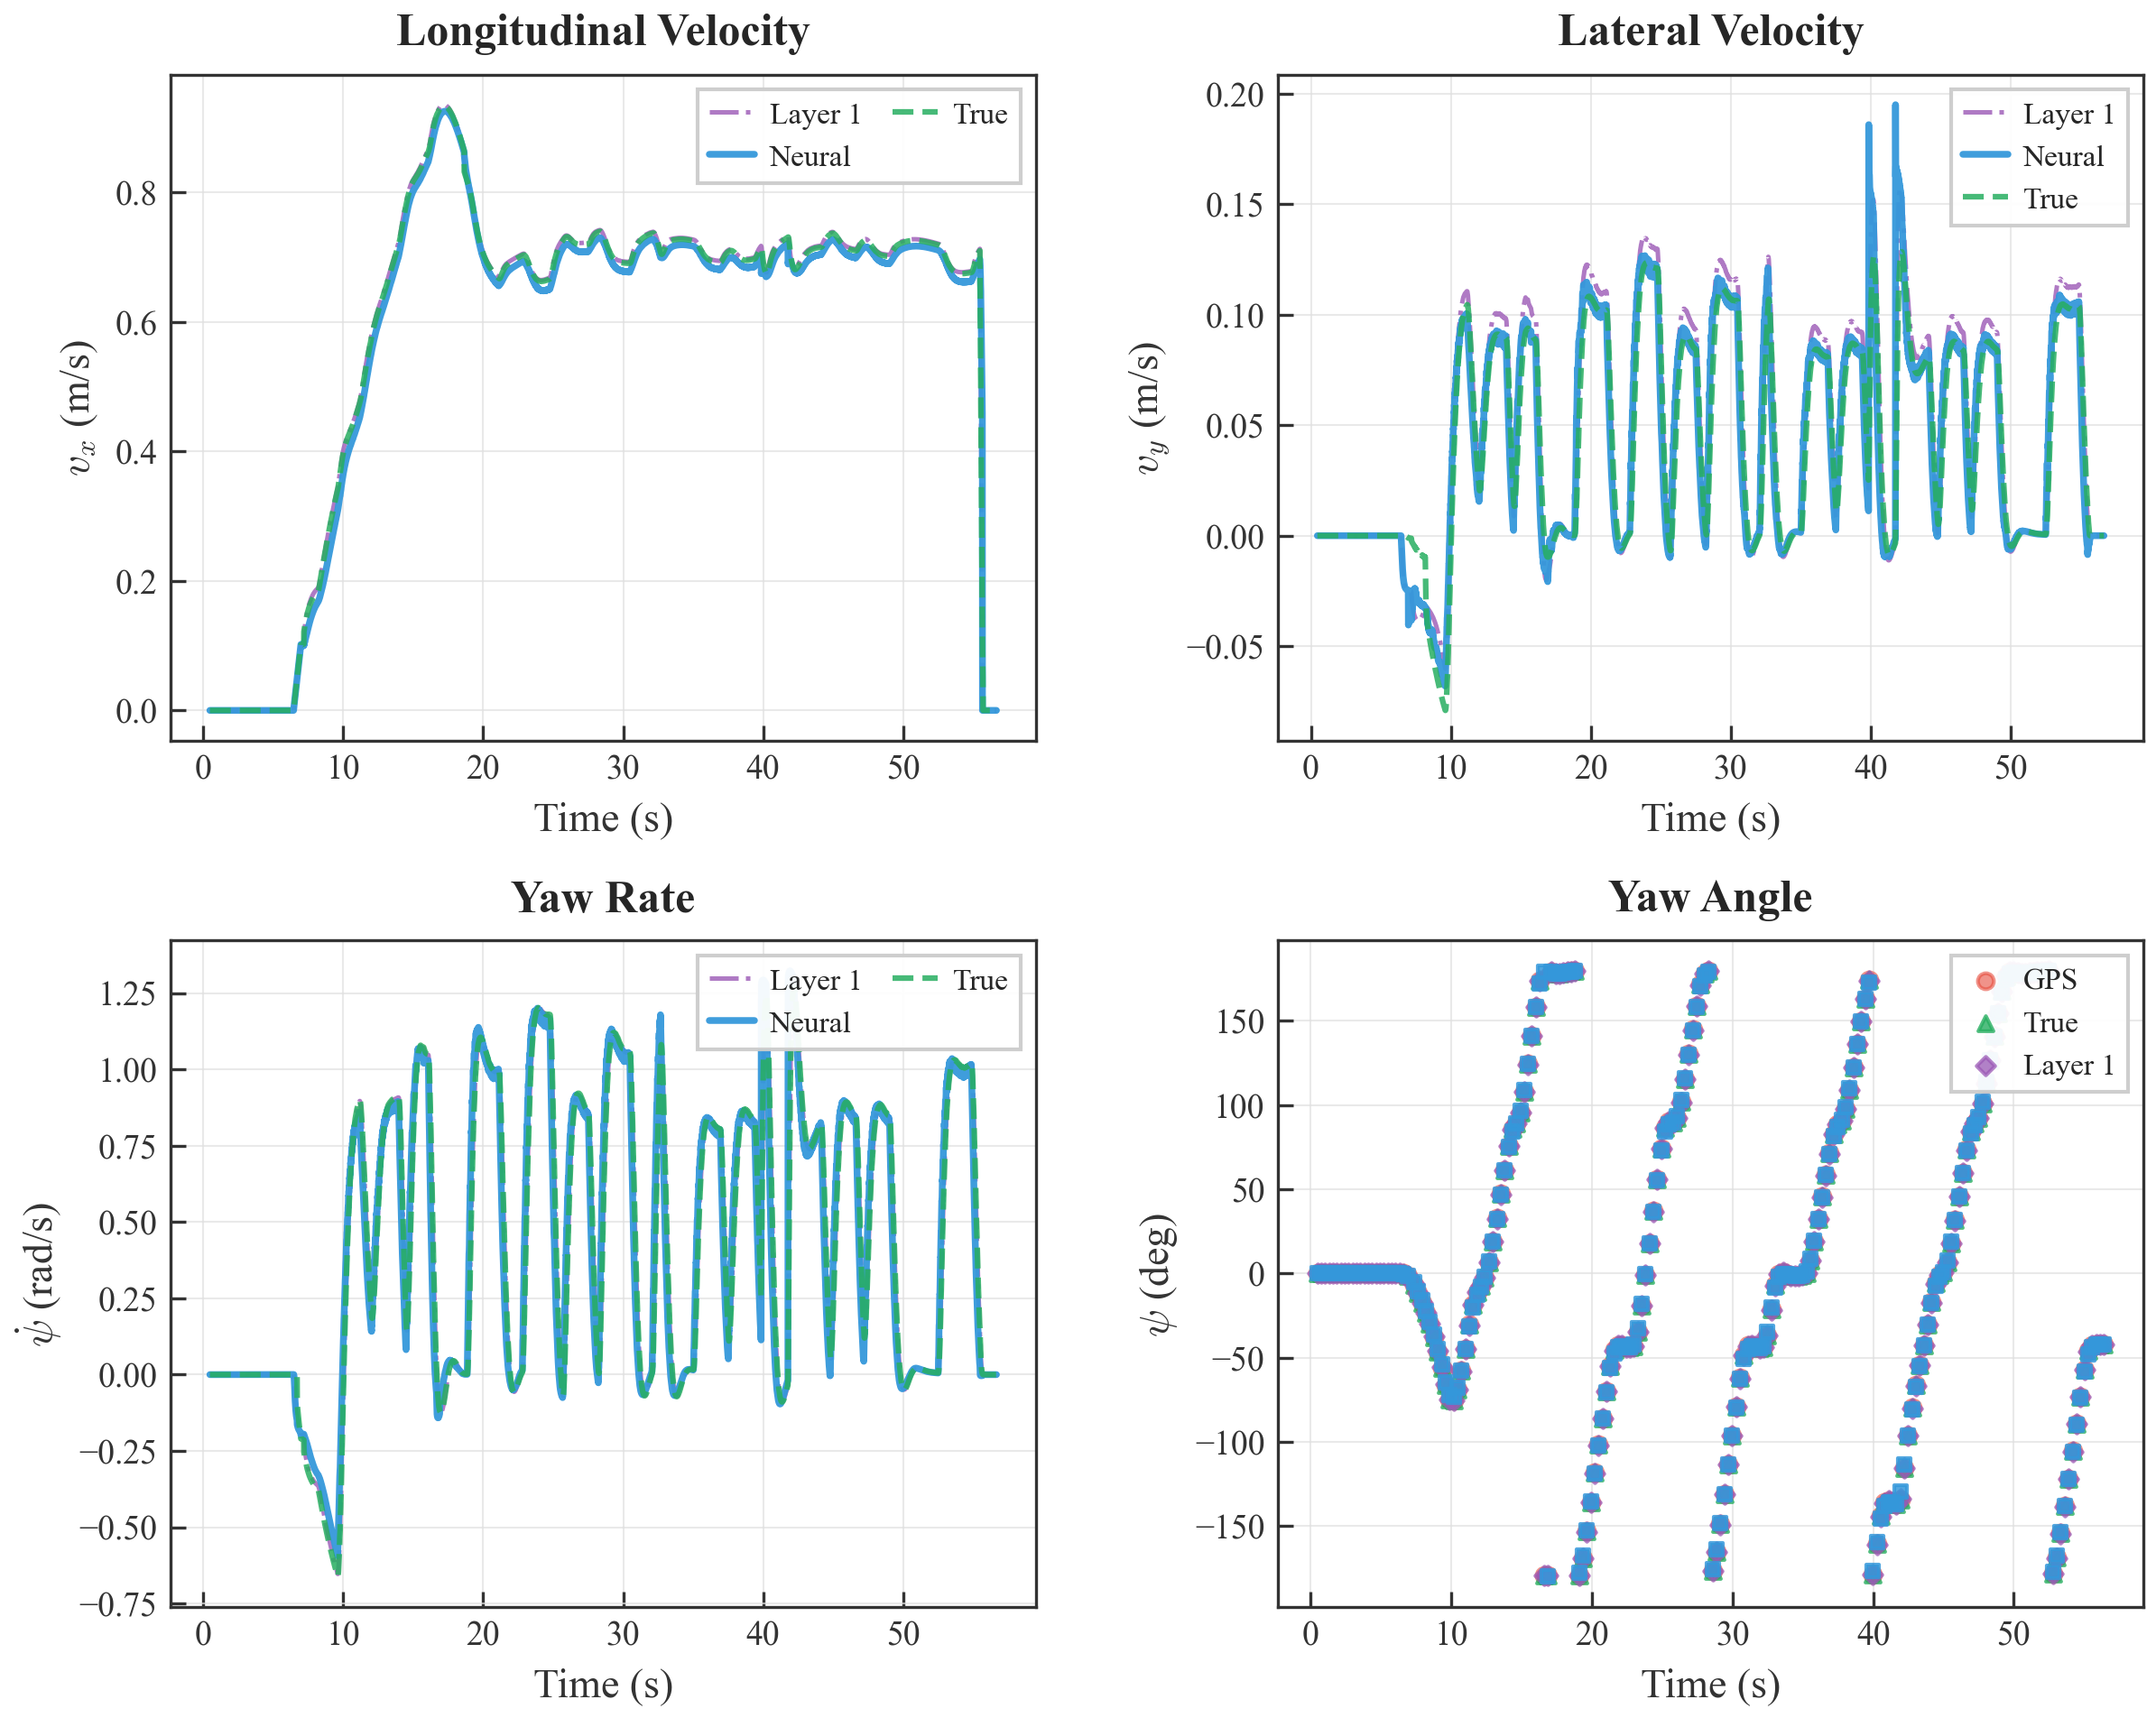
\includegraphics[width=0.96\linewidth,height=0.65\textheight,keepaspectratio]{State_est_py.png}
  \end{column}
  \begin{column}{0.27\textwidth}
    \vspace{0.20cm}
    \small
    \begin{block}{What matters}
      \begin{itemize}
        \item Measured states remain consistent with their sensor channels.
        \item The estimator supplies $v_y$, which is absent from $y$.
        \item The learned observer refines transient performance beyond its certified teacher.
      \end{itemize}
    \end{block}
  \end{column}
\end{columns}
\speakernote{
  \textbf{Memory cue:} Measured states stay consistent; the estimator supplies the state that sensors do not give.\par\smallskip
  This slide shows the individual state estimates. The measured channels remain consistent with their sensor signals. More importantly, the estimator reconstructs the lateral velocity $v_y$, which is not part of the measurement vector.\par\smallskip
  The lateral-velocity plot is a useful test of the hybrid approach because its dynamics are affected by uncertain tire forces. The UIO provides the stable baseline and the neural layer refines the transient behaviour. The yaw-rate and yaw-angle plots convey the same overall message: the observer follows nonlinear vehicle motion while maintaining output consistency. This reconstruction is then reflected in the tire-force residual estimates.
}
\end{frame}

% -----------------------------------------------------------------------------
\begin{frame}{Residual learning improves tire-force reconstruction}
\begin{columns}[T,onlytextwidth]
  \begin{column}{0.69\textwidth}
    \centering
    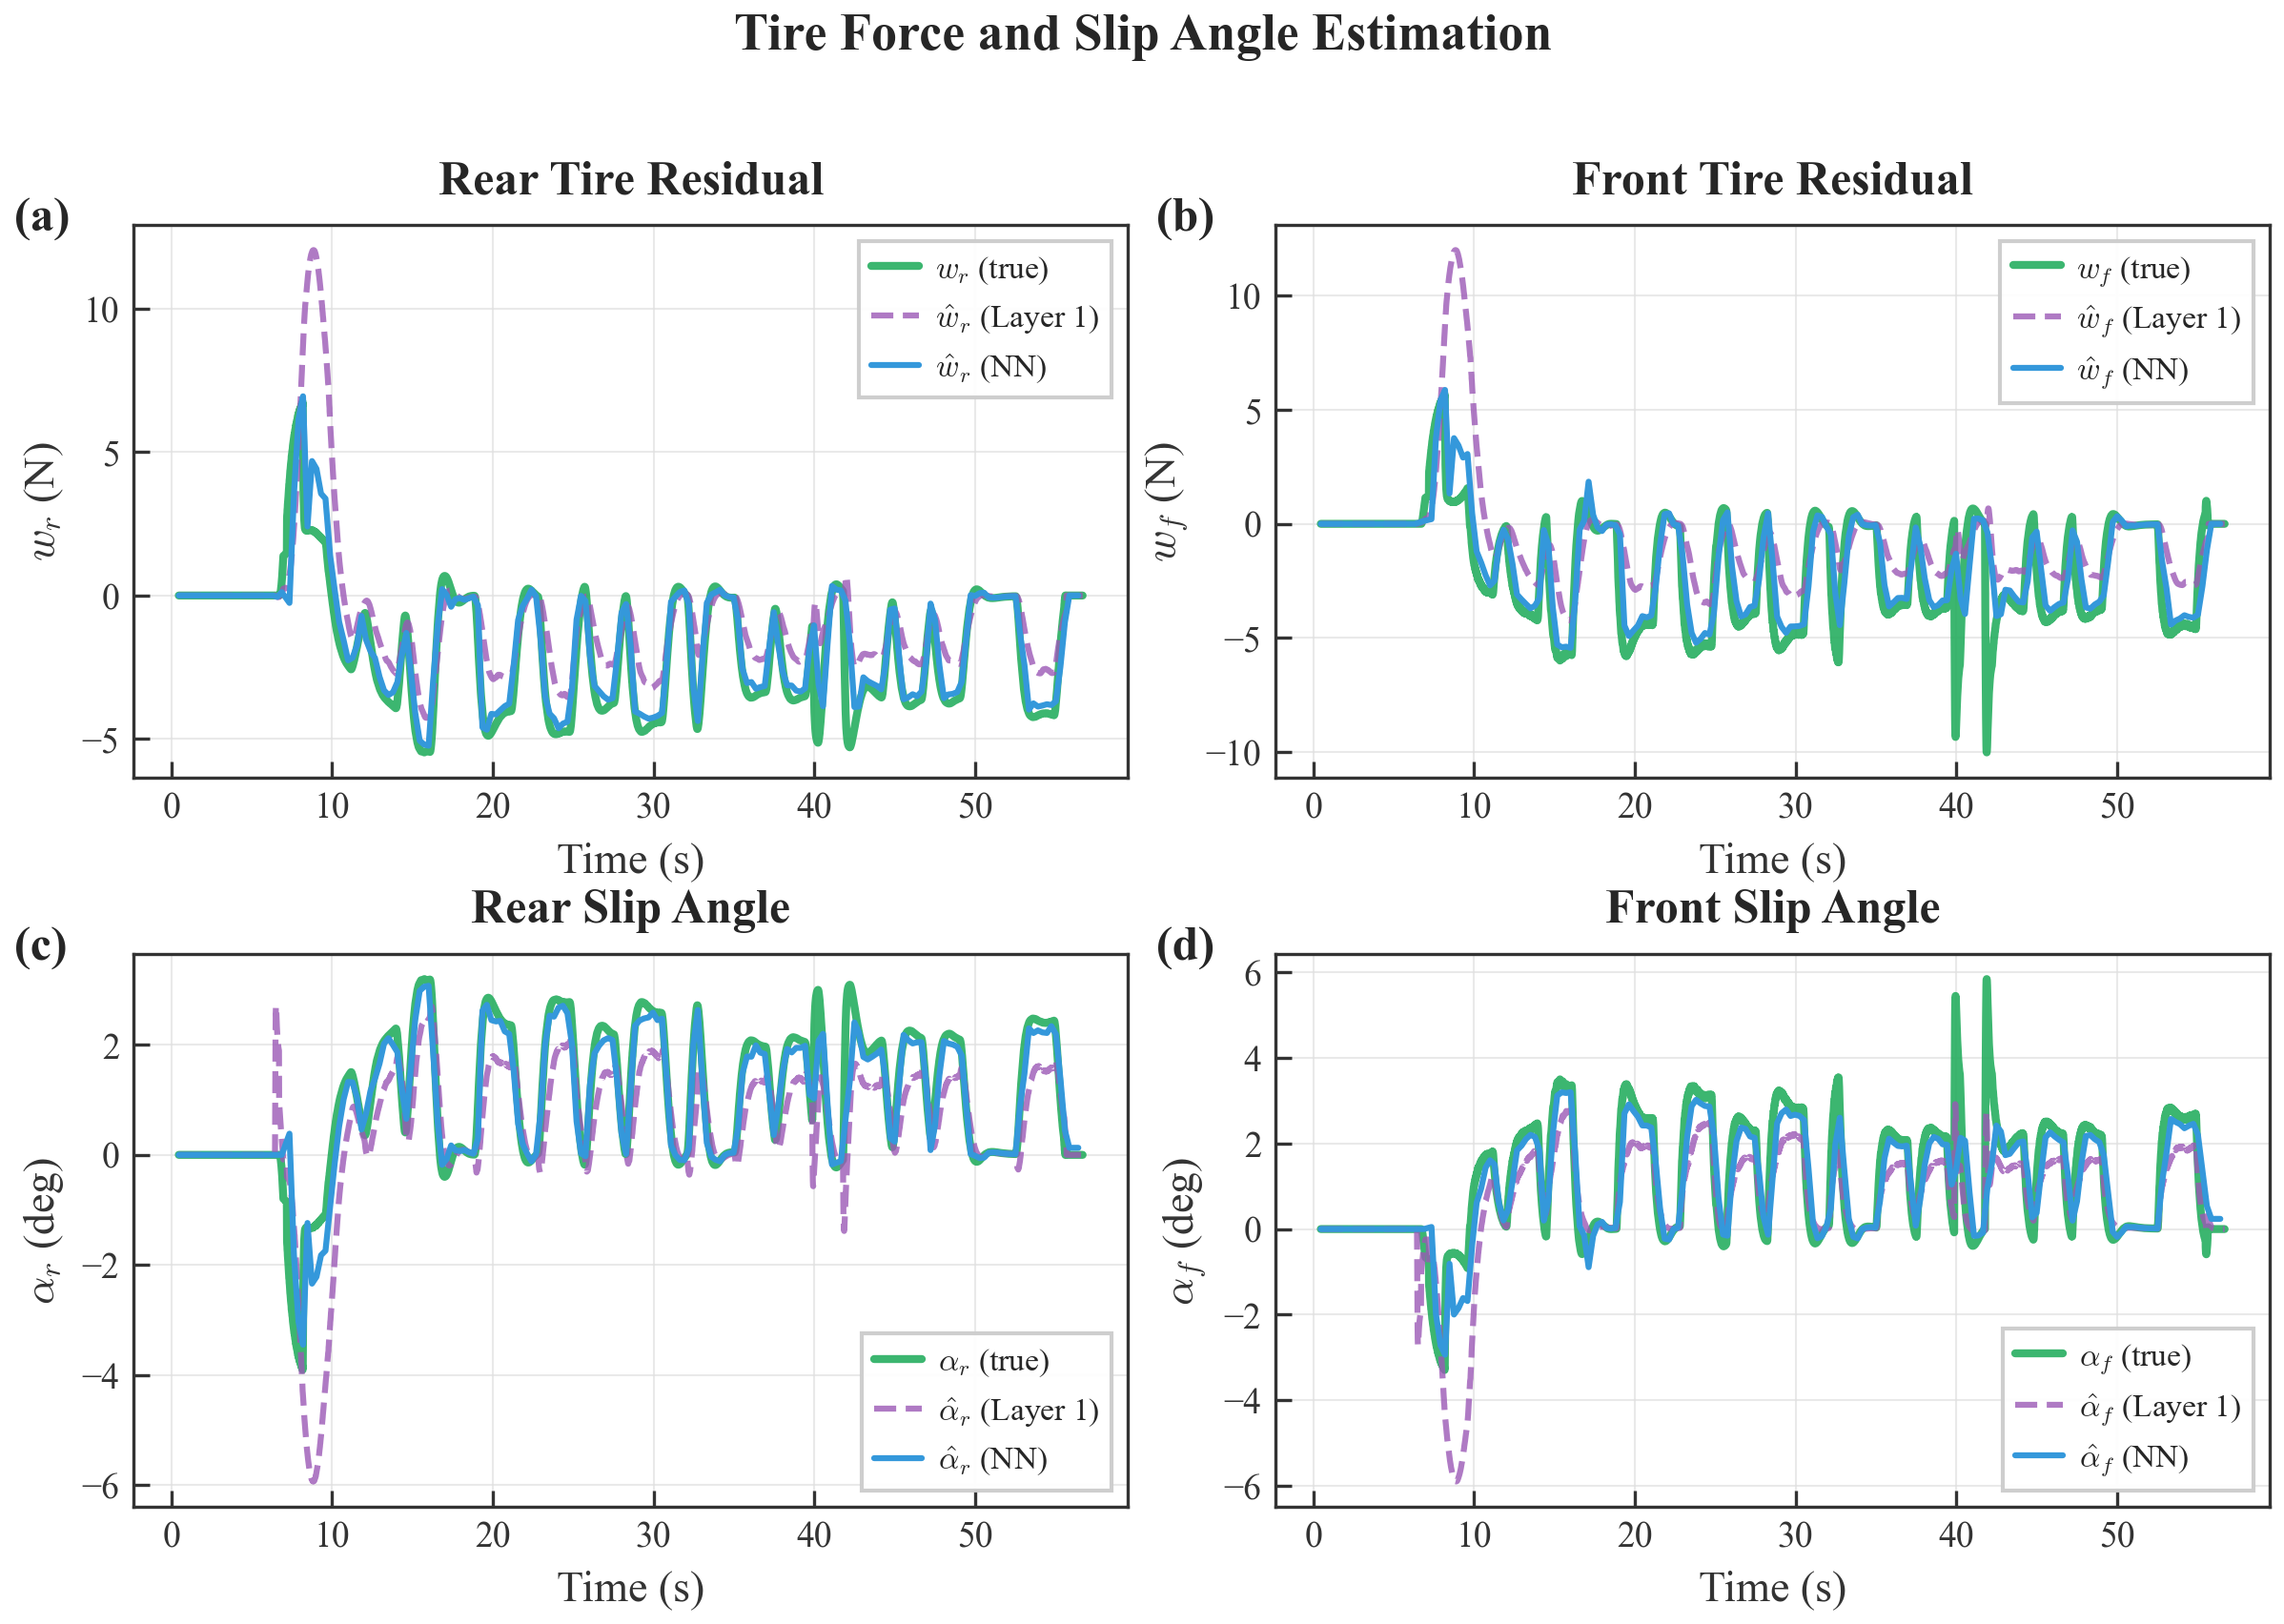
\includegraphics[width=0.96\linewidth,height=0.72\textheight,keepaspectratio]{tireforce_slip_py.png}
  \end{column}
  \begin{column}{0.27\textwidth}
    \vspace{0.18cm}
    \small
    \begin{block}{Interpretation}
      \begin{itemize}
        \item Layer 1 gives a bounded, physically meaningful residual estimate.
        \item Layer 2 converges faster and tracks tire-force residuals more closely.
        \item The learned map captures state-dependent residual dynamics.
      \end{itemize}
    \end{block}
  \end{column}
\end{columns}
\speakernote{
  \textbf{Memory cue:} The teacher is bounded; the student is faster and closer.\par\smallskip
  Finally, these plots compare the reconstructed tire-force residuals and slip angles. Layer 1 already gives a bounded and physically meaningful residual estimate. That is valuable by itself, because it turns an unknown modelling effect into an interpretable signal.\par\smallskip
  Layer 2 improves this estimate. The neural adaptive observer converges faster and tracks the front and rear tire-force residuals more closely over the manoeuvre. This is what we expect from a state-dependent residual model: the neural map can adapt to nonlinear effects that a fixed observer gain and nominal physics cannot capture completely. It refines, rather than replaces, the certified model-based estimate.
}
\end{frame}

% -----------------------------------------------------------------------------
\begin{frame}{Key takeaways}
\vspace{0.05cm}
\small
\begin{enumerate}
  \item \textbf{Relaxed UIO design:} regularization and output derivatives remove reliance on exact unknown-input decoupling.
  \vspace{0.18cm}
  \item \textbf{Certified robustness:} LMIs provide an explicit $\Hone$ bound for the generalized observer and an $\Ltwo$ bound for the neural observer.
  \vspace{0.18cm}
  \item \textbf{Reliable learning:} the UIO supplies stable supervisory signals; the neural observer learns the residual dynamics online.
  \vspace{0.18cm}
  \item \textbf{Vehicle evidence:} accurate trajectory tracking, recovery of the unmeasured lateral state, and improved tire-force estimates.
\end{enumerate}
\vspace{0.20cm}
\begin{block}{Central message}
  \centering\normalsize
  Certification and learning are complementary: the observer makes adaptation trustworthy,
  and adaptation makes the observer more accurate.
\end{block}
\speakernote{
  \textbf{Memory cue:} Relax the rank condition, certify the baseline, then learn the residual.\par\smallskip
  Let me conclude with four takeaways. First, the generalized unknown-input observer relaxes the need for exact unknown-input decoupling by using regularization and output derivatives. Second, the method keeps analytical guarantees: the first layer has an $\mathcal H^1$ robustness bound, and the neural observer has an $\mathcal L_2$ performance bound.\par\smallskip
  Third, the learning stage is guided by a certified teacher rather than being trained in isolation. This makes the learning signals more reliable and preserves physical interpretability. Finally, in the nonlinear vehicle example, the architecture achieves accurate trajectory tracking, reconstructs the unmeasured lateral velocity, and improves tire-force residual estimation. Certification and learning should work together: the observer makes adaptation trustworthy, and adaptation makes the observer more accurate. Thank you for your attention. I would be happy to take your questions.
}
\end{frame}

\end{document}
